% SCRIPT
% The next project in my presentation is named "Physician software interface for an intelligent glucose monitor."

%\renewcommand{\Titulo}{Physician software interface for an intelligent glucose monitor~}

\begin{frame}{\citetitle{MarcoNuno_CongArbIng_2012_01_00}\footnotemark (1)}

% Slide 1
\note[item]{\scriptsize Patients with type 1 or 2 diabetes require checking their blood glucose level several times a day. } 
%\note[item]{\scriptsize A portable glucose monitor measures glucose levels, some of them can store a history of glucose lectures}
%\note[item]{\scriptsize BGM have programmable alarms and a few of them can send data to a computer using Bluetooth or USB protocol. }
\note[item]{\scriptsize A device able to advise insulin doses based on physiological parameters of the patient and the number of carbohydrates to be ingested can be of great value in the assessment and treatment of patients having Diabetes. }
\note[item]{\scriptsize We developed a medical surveillance platform with two components}
\note[item]{\scriptsize The first component is an Intelligent Glucose Monitor (IGM)
with the hardware layer and electronics needed to interact with glucose-sensing strips}
\note[item]{\scriptsize The second one is a Physician software interface (PSI) to configure and extract information from an Intelligent Glucose Monitor (IGM). }

\begin{block}{Description} 
	\begin{itemize}
\item Patiens with Diabetes requires checking their blood glucose level (BCL) several times in a day
\item Most of the commercial Blood Glucose Monitors (BGM) store an history of patient's BCL.
\item We developed an Intelligent Glucose Monitor (IGM).
\item Data can be obtained on a PC using a physician software interface (PSI).
\item Tools:
	\begin{itemize}
		\item C++ for the IGM.
		\item Java for the PSI.
	\end{itemize}
	\end{itemize}
\end{block} 
\footnotetext[1]{\fullcite{MarcoNuno_CongArbIng_2012_01_00}}
\setcounter{footnote}{0}
\end{frame}

\begin{frame}{\citetitle{MarcoNuno_CongArbIng_2012_01_00} (2)}
% Slide 2
\note[item]{\scriptsize On the right top, we show the hardware components of the proposed IGM. In the right button, we show an image of the first prototype of the IGM. A menu was to allow the user to obtain as many blood glucose levels as desired. The user selects the menu option by pressing the red keys in the IGM front, obtained from a TV remote control.}

\begin{block}{Proposed System (Hardware)} 
\begin{columns}
		\begin{column}{0.48\textwidth}
		    Components of the IGM
		    \begin{itemize}
		        \item Microcontroller.
                \item LCD Display.
                \item Glucose sensor.
                \item Real time clock.
                \item USB interface.
                \item Interface to connect glucose-sensing strips.
            \end{itemize}
            A simple menu system shown in the LCD screen allows the user to interact with the IGM. 
		\end{column}
		
				\begin{column}{0.48\textwidth}
\begin{center}
     \begin{tabular}{c}
         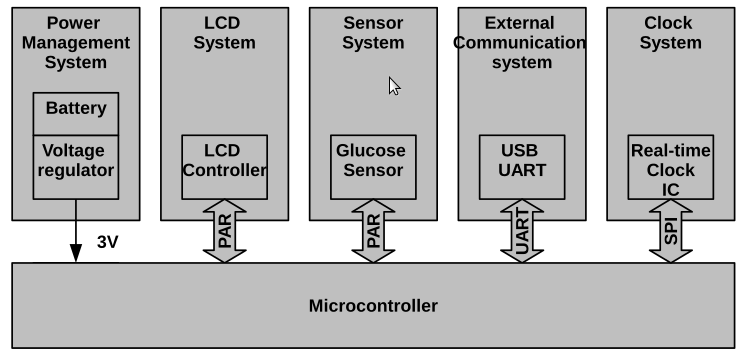
\includegraphics[width=0.85\linewidth]{Figs/IntelligentGlucometer1}\\
         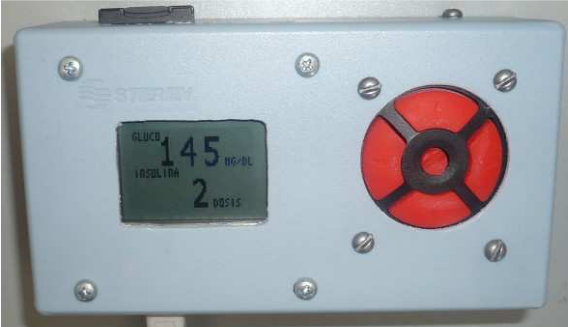
\includegraphics[width=0.75\linewidth]{Figs/IntelligentGlucometer3}\\
          \end{tabular}
\end{center}
		\end{column}
				\end{columns}

\end{block} 
\end{frame}



\begin{frame}{\citetitle{MarcoNuno_CongArbIng_2012_01_00} (3)}
\begin{block}{Proposed System (PSI Software)}

% SLide 4
%\note[item]{\scriptsize The PSI is designed to allow physician to communicate with the IGM in order to extract information contained into the device and perform configuration tasks. } 
% Conclusion
\note[item]{Whole system was used by fifteen patients under observation by two treating physicians in the Children’s Hospital of Tamaulipas (CHT). }
\note[item]{Several improvements are pending: replace the PC-based PSI by a smarphone or tablet device. To reduce the dimentions of the IGM, and to add a touch LCD screen to improve the interface.  }




\begin{columns}
		\begin{column}{0.48\textwidth}
		The designed PC-based PSI allows the pysician the following actions: 
		\begin{itemize}
		\item To obtain and store data of the IGM, and generate reports related to the BGL.
		\item To configure patient's insuline profile.
		
        \end{itemize}
				\end{column}
				\begin{column}{0.48\textwidth}
\begin{center}
     \begin{tabular}{c}
         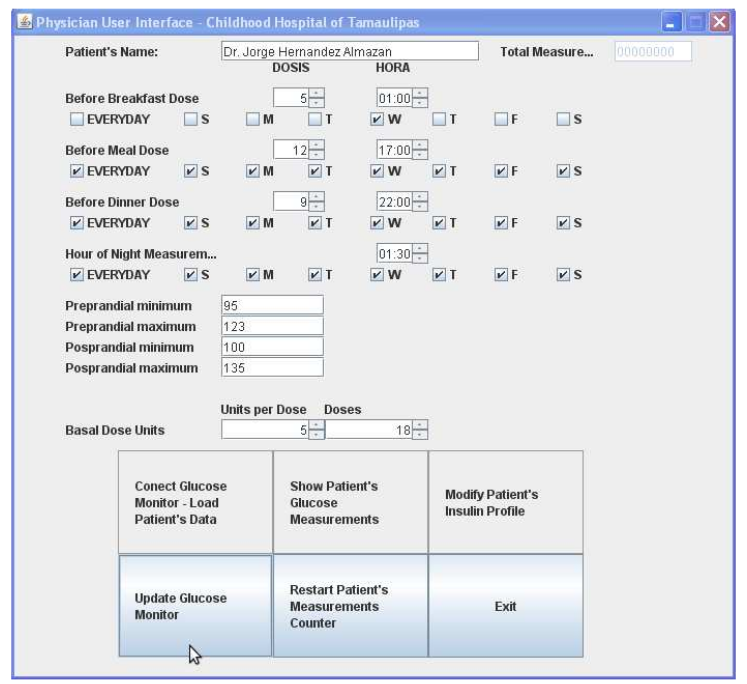
\includegraphics[width=0.86\textwidth]{Figs/IntelligentGlucometer4}
          \end{tabular}
\end{center}
		\end{column}
				\end{columns}
\end{block} 
\end{frame}


